\Subsection{Система множеств}
Полезные обозначения: $A \sqcup B$ - объединение $A$ и $B$, такие что $A \cap B = \emptyset$

\begin{definition}
    Набор мн-в дизъюнктный, если мн-ва попарно не пересекаются: $\bigsqcup_{\alpha \in I}A_{\alpha}$
\end{definition}

\begin{definition}
    $E$ -- мн-во; если $E = \bigsqcup_{\alpha \in I} E_{\alpha}$ -- разбиение мн-ва $E$.
\end{definition}

Напоминание:
$$X \setminus \bigcup_{\alpha \in I} A_{\alpha} = \bigcap X \setminus A_{\alpha}$$
$$X \setminus \bigcap_{\alpha \in I} A_{\alpha} = \bigcup X \setminus A_{\alpha}$$


\begin{definition}
    $\mathcal{A}$ -- система подмн-в $X$: $A \subset 2^{X}$

    \begin{enumerate}
        \item ($\delta_0$): если $\forall A, B \in \mathcal{A} \implies A \cap B \in \mathcal{A}$
        \item ($\sigma_0$): если $\forall A, B \in \mathcal{A} \implies A \cup B \in \mathcal{A}$
        \item {
            $(\delta)$: если $A_n \in \mathcal{A}, \ \forall n \implies \bigcap_{n=1}^{\infty} A_n \in \mathcal{A}$
        }
        \item {
            $(\sigma)$: если $A_n \in \mathcal{A}, \ \forall n \implies \bigcup_{n=1}^{\infty} A_n \in \mathcal{A}$
        }
    \end{enumerate}
\end{definition}

\begin{definition}
    $\mathcal{A}$ -- симметрическая система мн-в, если $\forall A \in \mathcal{A} \implies X \setminus A \in \mathcal{A}$.
\end{definition}

\begin{statement}
    Если $\mathcal{A}$ -- симм., то $(\delta_{0}) \Leftrightarrow (\sigma_{0})$ и $(\delta) \Leftrightarrow (\sigma)$.
\end{statement}

\begin{proof}
    $A_{\alpha \in I}\mathcal{A} \Leftrightarrow X \setminus A_{\alpha} \in \mathcal{A} \implies \bigcup_{\alpha \in I}A_{\alpha} = \bigcap_{\alpha \in I} X \setminus A_{\alpha} \in \mathcal{A}$
\end{proof}

\begin{definition}
    $\mathcal{A}$ -- алгебра мн-в, если $\mathcal{A}$ -- симметр., $\emptyset \in \mathcal{A}$ и $\forall A, \ B \in \mathcal{A}: \ A \cup B \in \mathcal{A}$ (по утв. 1.1 $(\delta_0) \Leftrightarrow (\sigma_0)$; смотри \href{https://ru.wikipedia.org/wiki/%D0%90%D0%BB%D0%B3%D0%B5%D0%B1%D1%80%D0%B0_%D0%BC%D0%BD%D0%BE%D0%B6%D0%B5%D1%81%D1%82%D0%B2#%D0%9E%D0%BF%D1%80%D0%B5%D0%B4%D0%B5%D0%BB%D0%B5%D0%BD%D0%B8%D0%B5}{опр. алгебры}).
\end{definition}

\begin{properties}
    алгебры мн-в: 

    \begin{enumerate}
        \item {
            $\emptyset, X \in \mathcal{A}$
        }
        \item Если $A_1, \dots, A_n \in \mathcal{A}$, то $\bigcup_{k = 1}^n A_k \in \mathcal{A} \land \bigcap_{k = 1}^n A_k \in \mathcal{A}$
        \item Если $A, B \in \mathcal{A}$, то $A \cap (X \setminus B) = A \setminus B \in \mathcal{A}$
    \end{enumerate}
\end{properties}

\begin{definition}
    $\mathcal{A}$ - \sigma-алгебра мн-в, если $\mathcal{A}$ -- симм., $\emptyset \in \mathcal{A}$ и свойство (\sigma) выполнено (т.е. есть замкнутость по объединению любого числа множетсв; в силу симметричности по утв. 1.1 получаем $(\sigma) \Leftrightarrow (\delta)$).
\end{definition}

\begin{remark}
    \sigma-алгебра $\implies$ алгебра.
\end{remark}

\begin{example}
    \begin{enumerate}
        \item $2^X$ - \sigma-алгебра.
        
        \item $X = \mathbb{R}^2$, $\mathcal{A}$ - всевозможные \href{https://ru.wikipedia.org/wiki/%D0%9E%D0%B3%D1%80%D0%B0%D0%BD%D0%B8%D1%87%D0%B5%D0%BD%D0%BD%D0%BE%D1%81%D1%82%D1%8C}{огр. подмн-ва.} $\mathbb{R}^2$ и их дополнения. ($\mathcal{A}$ -- алгебра, но не \sigma-алгебра).
        
        \textbf{Rem}: огр. множество - в метрич. пр-ве это множетсво ограниченного диаметра ($d(x, \ y) := || x - y ||$), т.е. $sup\{ d(x, \ y) \ | x, \ y \in X \}$ - ограничен.

        \item $\mathcal{A}$ - алгебра (\sigma-алгебра) подмн-в $X$ и $Y \subset X$. $\mathcal{A}_{Y} := \{A \cap Y : A \in \mathcal{A}\}$ -- индуцированная алгебра (\sigma-алгебра).
        
        \item Пусть $\mathcal{A}_{\alpha}$ -- алгебры (\sigma-алгебры), тогда $\bigcap_{\alpha \in I}\mathcal{A}_{\alpha}$ -- алгебра (\sigma-алгебра).
        
        \item $A, B \subset X$ ниже перечислено, что есть в алгебре, содержащей $A, B$: \\ $\emptyset, X, A, B, A \cup B, A \cap B, A \setminus B, B \setminus A, X \setminus A, X \setminus B, X \setminus (A \cup B), X \setminus (A \cap B), A \vartriangle B, X \setminus (A \vartriangle B), X \setminus (A \setminus B), X \setminus (B \setminus A)$.
    \end{enumerate}
\end{example}

\begin{theorem}
    Пусть $\epsilon$ -- семейство подмн-в в $X$, тогда существует наименьшая по включению \sigma-алгебра (алгебра) $\mathcal{A}$, такая что $\epsilon \subset \mathcal{A}$.
\end{theorem}

\begin{proof}
    $\mathcal{A}_{\alpha}$ -- всевозможные \sigma-алгебры $\supset \epsilon$. Такие есть, так как $2^X$ подходит.

    $\mathcal{A} := \bigcap_{\alpha \in I} \mathcal{A}_{\alpha} \supset \epsilon$. Теперь проверим, что $\mathcal{A}$ -- наим. по вкл. $\mathcal{A} \subset A_{\alpha}$ $\forall \alpha \in I$.

    \begin{definition}
        \begin{enumerate}
            \item Такая \sigma-алгебра -- борелевская оболочка $\epsilon$ -- $(\mathcal{B}(\epsilon))$.
            
            \item $X = \mathbb{R}^n$; такая \sigma-алгебра, натянутая на все открытые мн-ва -- борелевская \sigma-алгебра $(\mathcal{B}^n)$.
        \end{enumerate}
    \end{definition}

    \begin{remark}
        $\underbrace{\mathcal{B}^n}_{\text{континуальное}} \neq \underbrace{2^{\mathbb{R}^n}}_{\text{больше континуального}}$
    \end{remark}
\end{proof}

\begin{definition}
    $R$ -- кольцо, если $\forall A, B \in R \implies A \cup B, A \cap B, A \setminus B \in R$.
\end{definition}

\begin{remark}
    Кольцо + $(X \in R) \implies$ алгебра.
\end{remark}

\begin{definition}
    $P$ -- полукольцо, если 
    \begin{enumerate}
        \item $\emptyset \in P$
        \item $\forall A, B \in P \implies A \cap B \in P$
        \item $\forall A, B \in P \implies \exists Q_1, Q_2, \dots, Q_n \in P$, такие что $A \setminus B = \bigsqcup_{k = 1}^{n}Q_k$.
    \end{enumerate}
\end{definition}

\begin{example}
    $X = \mathbb{R}, P = \{(a, b] : a, b \in X\}$ -- полукольцо.

    \hbox{
        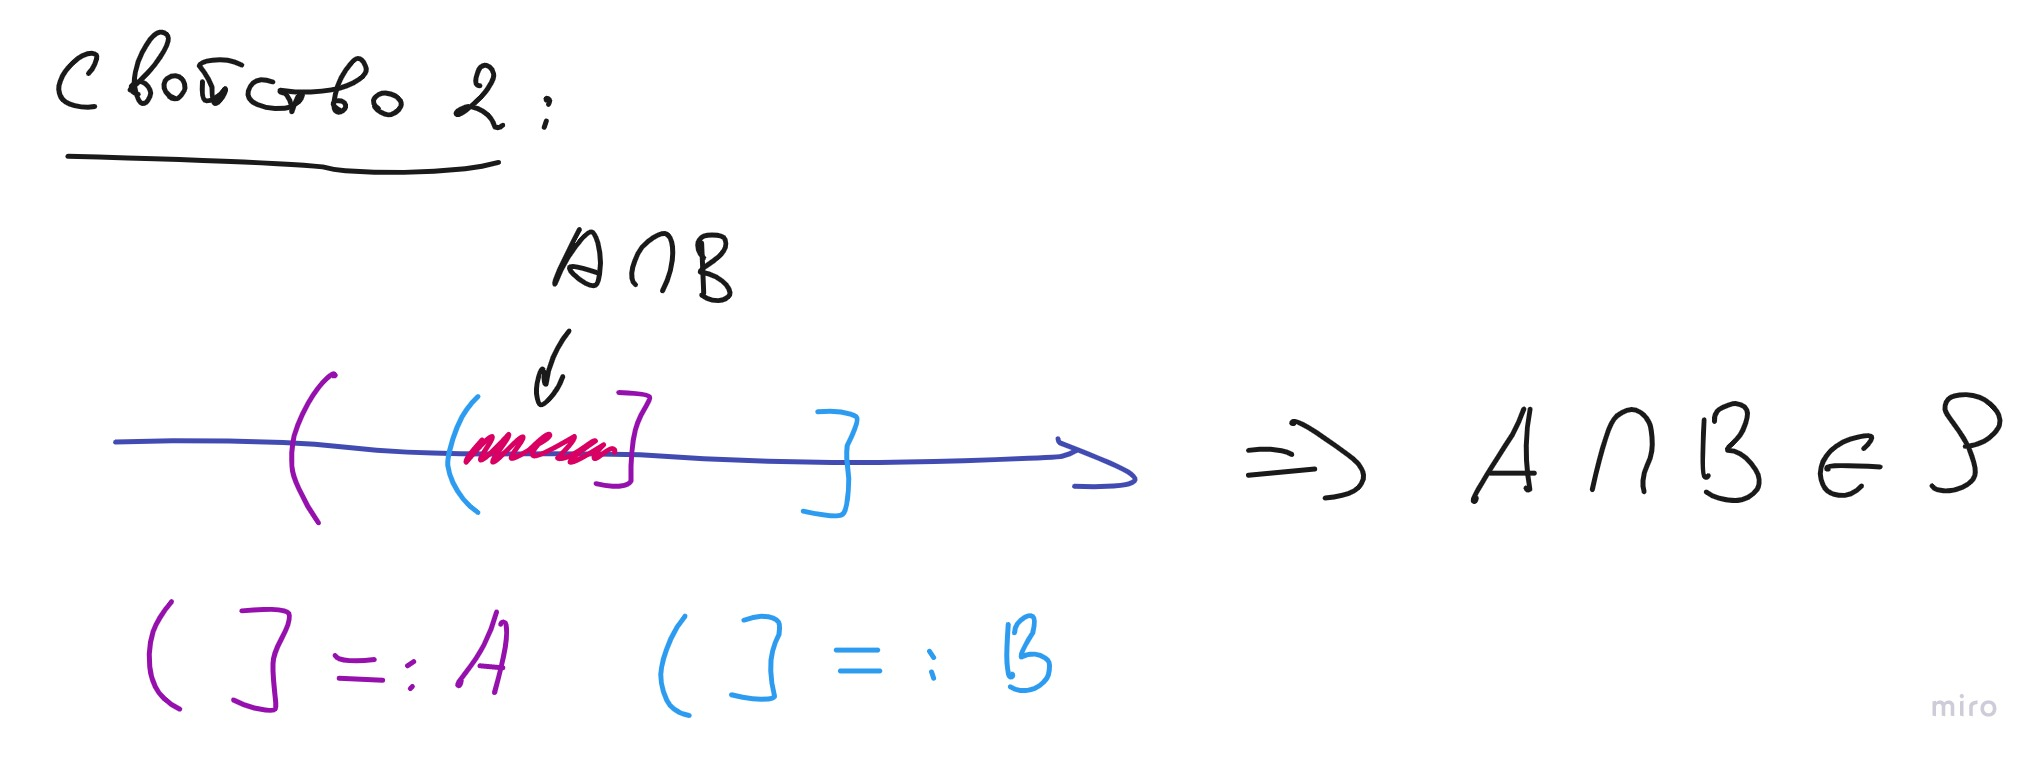
\includegraphics[scale=0.15]{./assets/01-measure-theory/semicircle-prop-2.jpg}
    }
    \hbox{
        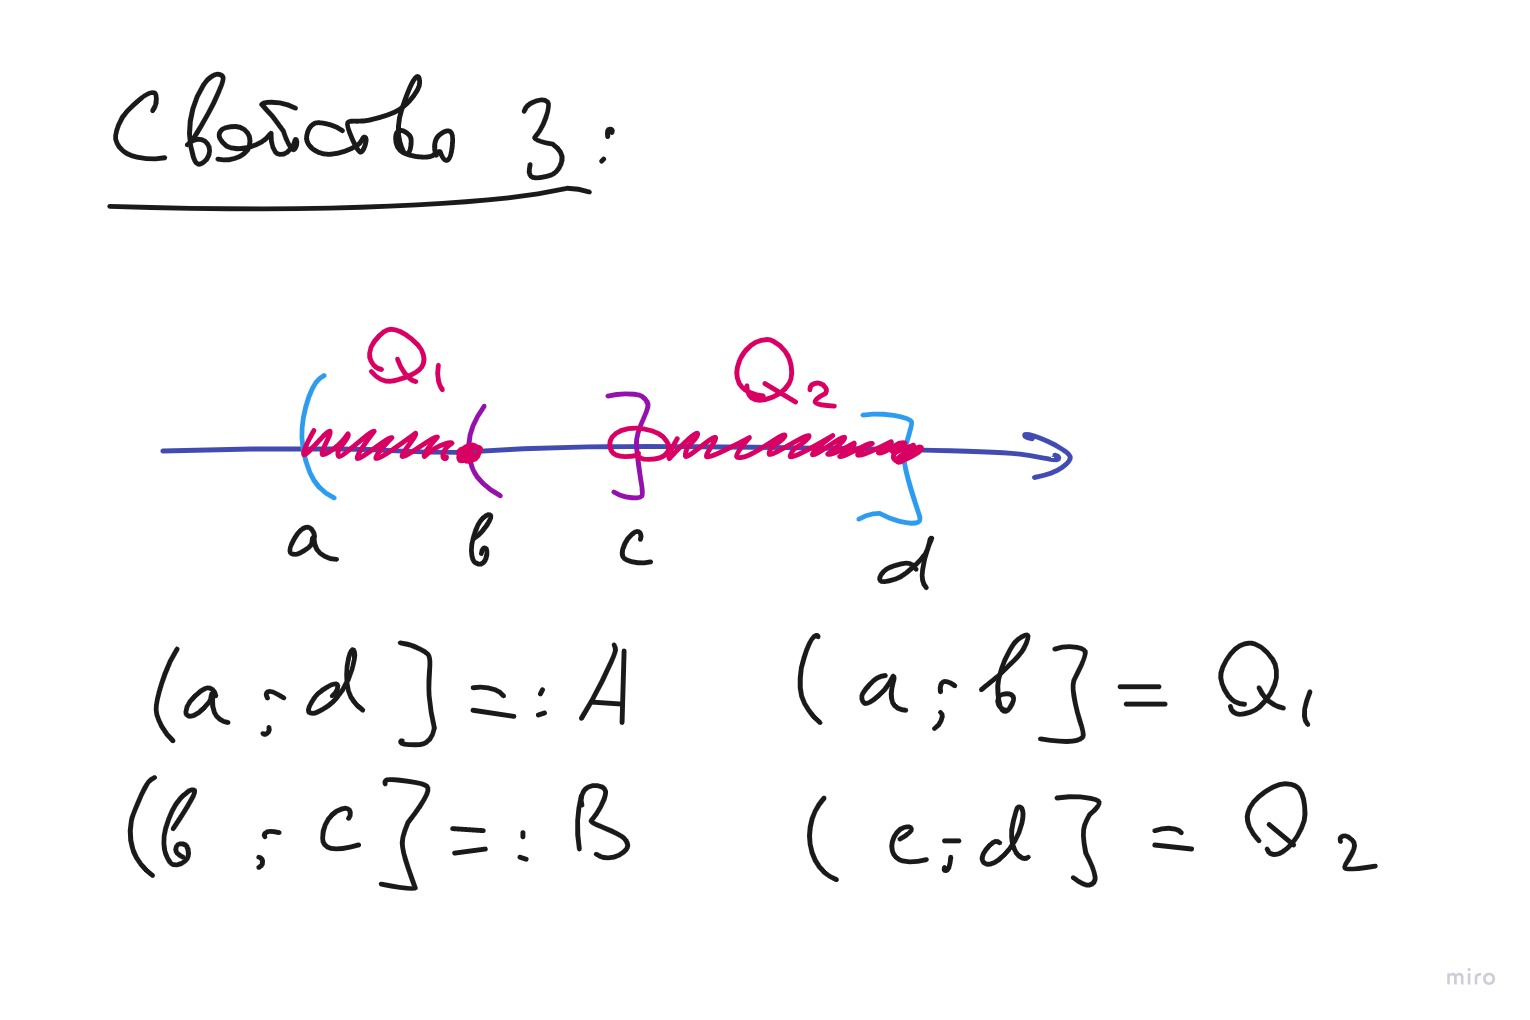
\includegraphics[scale=0.15]{./assets/01-measure-theory/semicircle-prop-3.jpg}
    }

\end{example}

\begin{lemma}
    $\bigcup_{n=1}^{N} A_n = \bigsqcup_{n=1}^{N}\underbrace{A_n \setminus \left(\bigcup_{k=1}^{n-1}A_k\right)}_{B_n}$.
\end{lemma}
\begin{proof}
    $\supset$: Дизъюнктивность $B_n \subset A_n $ и при $m > n$ $B_m \cap A_n = \emptyset \implies B_n \cap B_m = \emptyset$.
    
    $\subset$: Пусть $x \in \bigcup_{n=1}^{N} A_n$. Возьмем наим. $m$, такой что $x \in A_m \implies x \in B_m \implies x \in \bigsqcup_{n=1}^{N} B_n$.
\end{proof}

\begin{theorem}
    $P, P_1, P_2, \dots \i \mathcal{P}$. Тогда 

    \begin{enumerate}
        \item $P \setminus \bigcup_{k=1}^{n} P_k = \bigsqcup_{j=1}^m Q_j$, где $Q_j \in \mathcal{P}$ -- полукольцо.
        \item $\bigcup_{k=1}^{n} P_k = \bigsqcup_{k=1}^{n} \bigsqcup_{j=1}^{m_k} Q_{kj}$, где $Q_{kj} \in \mathcal{P}$ и $Q_{kj} \subset P_k$. 
    \end{enumerate}
\end{theorem}

\begin{proof}
    \begin{enumerate}
        \item индукция по n. База -- опр. полукольца. Переход ($n \rightarrow n+1$): \\ $P \setminus \bigcup_{k=1}^{n+1}P_k = \left(P \setminus \bigcup_{k=1}^nP_k\right) \setminus P_{k+1} = \bigsqcup_{j=1}^{m} \left(\underbrace{Q_j \setminus P_{n+1}}_{\bigsqcup_{i=1}^{l_j}Q_{ji}}\right)$
        \item $\bigcup_{k=1}^{n} P_k = \bigsqcup_{k=1}^{n} \left(\underbrace{P_k \setminus \bigcup_{j=1}^{k-1} P_j}_{\bigsqcup_{j=1}^{m_k} Q_{kj}}\right)$
    \end{enumerate}
\end{proof}

\begin{remark}
    В (2) можно писать $n = \infty$.
\end{remark}

\begin{definition}
    $\mathcal{P}$ -- полукольцо подмн-ва $X$.

    $\mathcal{Q}$ -- полукольцо подмн-ва $Y$.

    $\mathcal{P} \times \mathcal{Q} := \{P \times Q : P \in \mathcal{P}, Q \in \mathcal{Q}\}$ -- декартово произведение полуколец.
\end{definition}

\begin{theorem}
    Декартово произведение полуколец -- полукольцо.
\end{theorem}
\begin{proof}
    
    $$(P \times Q) \cap (P' \times Q') = (P \cap P') \times (Q \cap Q')$$

    $$(P \times Q) \setminus (P' \times Q') = (P \setminus P') \times Q \sqcup (P \cap P') \times (Q \setminus Q')$$
\end{proof}

\begin{remark}
    Остальные структуры не сохр. при декартовом произведении: $2^X \times 2^Y$ -- полукольцо.
\end{remark}

\begin{definition}
    Замкнутый параллелепипед $a, b \in \mathbb{R}^m$.

    $[a, b] = [a_1, b_1] \times [a_2, b_2] \times \dots \times [a_m, b_m]$

    Открытый параллелепипед:

    $(a, b) = (a_1, b_1) \times (a_2, b_2) \times \dots \times (a_m, b_m)$

    Ячейка:
    
    $(a, b] = (a_1, b_1] \times (a_2, b_2] \times \dots \times (a_m, b_m]$
\end{definition}

\begin{theorem}
    Непустая ячейка -- перечисление убыв. посл. открытых паралл. / объединение возраст. послед. замкн.
\end{theorem}

\begin{proof}

    $P_n := (a_1, b_1 + \frac{1}{n}) \times \dots \times (a_m, b_m + \frac{1}{n})$

    $P_n \supset P_{n+1}$ и $\bigcap_{n=1}^{\infty}P_n = (a, b]$

    $Q_n := [a_1 + \frac{1}{n}, b_1] \times \dots \times [a_m + \frac{1}{n}, b_m]$

    $Q_n \subset Q_{n+1}$ и $\bigcup_{n=1}^{\infty}Q_n = (a, b]$ 

    \hbox{
        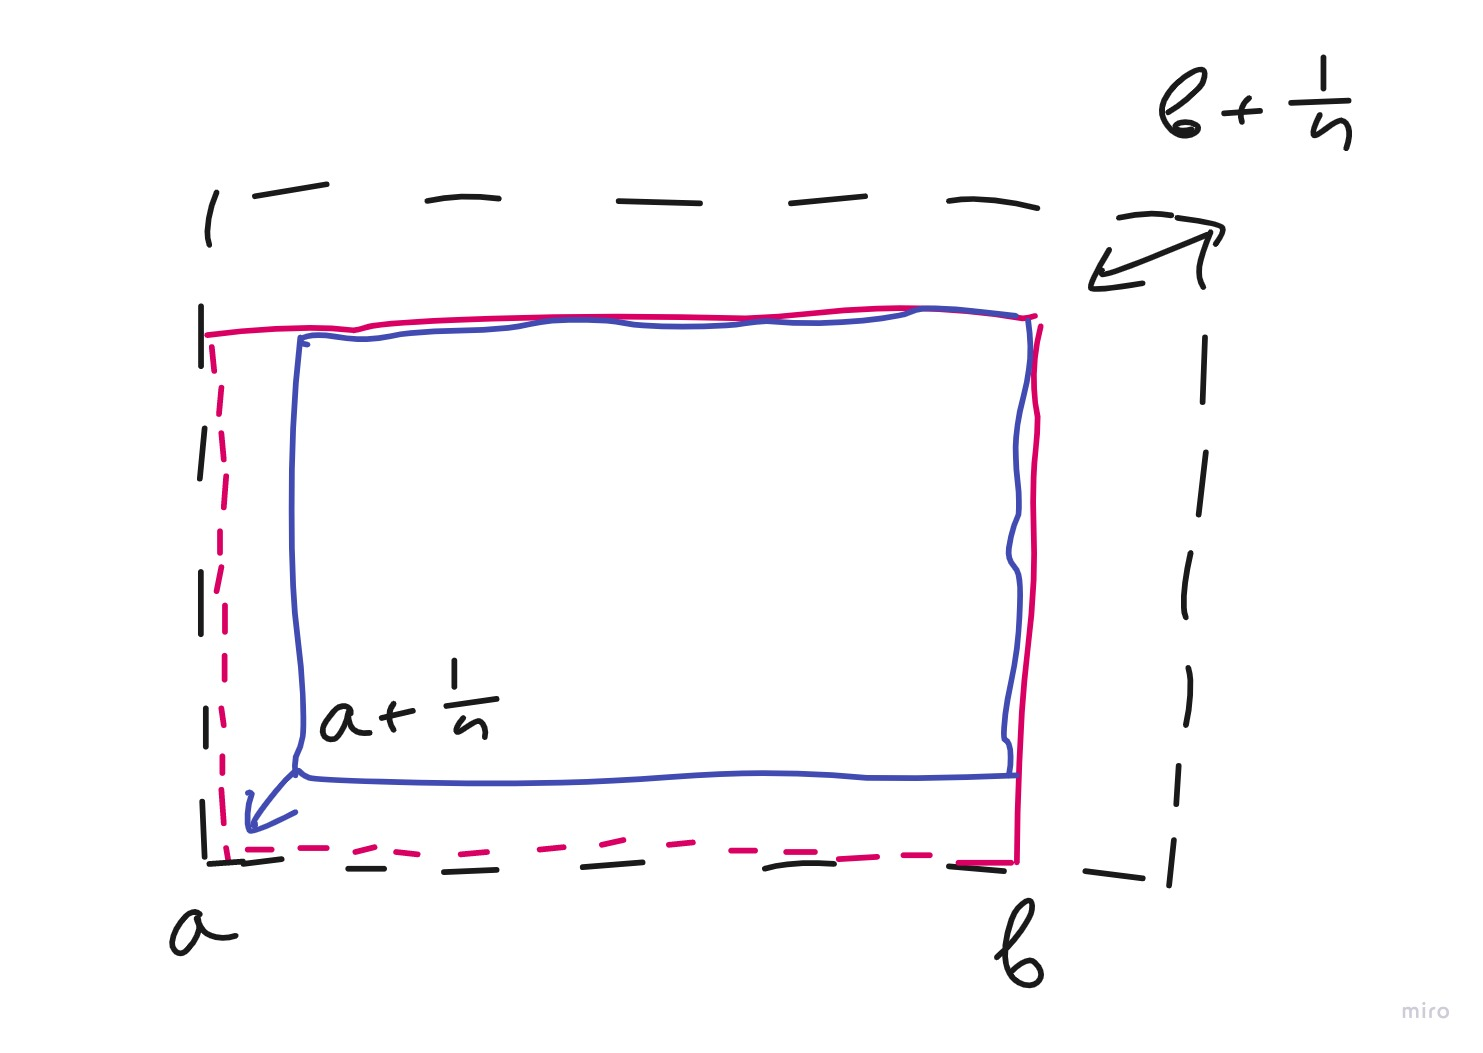
\includegraphics[scale=0.15]{./assets/01-measure-theory/rects-1.jpg}
    }

\end{proof}

\textbf{Обозначения}: $\mathcal{P}^m$ -- сем-во ячеек из $\mathbb{R}^m$.

$\mathcal{P}_{Q}^{m}$ -- сем-во ячеек из $\mathbb{R}^m$ с рациональными координатами вершин.

\begin{theorem}
    $\mathcal{P}^m, \mathcal{P}^m_Q$ -- полукольца.
\end{theorem}
\begin{proof}
    $\mathcal{P}^m = \mathcal{P}^{m-1} \times \mathcal{P}^1$

    $\mathcal{P}_Q^m = \mathcal{P}_Q^{m-1} \times \mathcal{P}_Q^1$
\end{proof}

\begin{theorem}
    $G \neq \emptyset$ -- открытое множество в $\mathbb{R}^m$. Тогда его можно представить как не более чем счетное дизъюнктивное объелинение ячеек, замыкание каждой из которых содержится в $G$ (можно считать, что ячейки с рациональными координатными вершинами).
\end{theorem}
\begin{proof}

    $R_x$ -- ячейка, $\underbrace{Cl  (R_x)}_{\text{замыкание ячейки}} \subset G$, $x \in R_x$, получаем, что $G = \bigcup_{x \in G} R_x$.

    \hbox{
        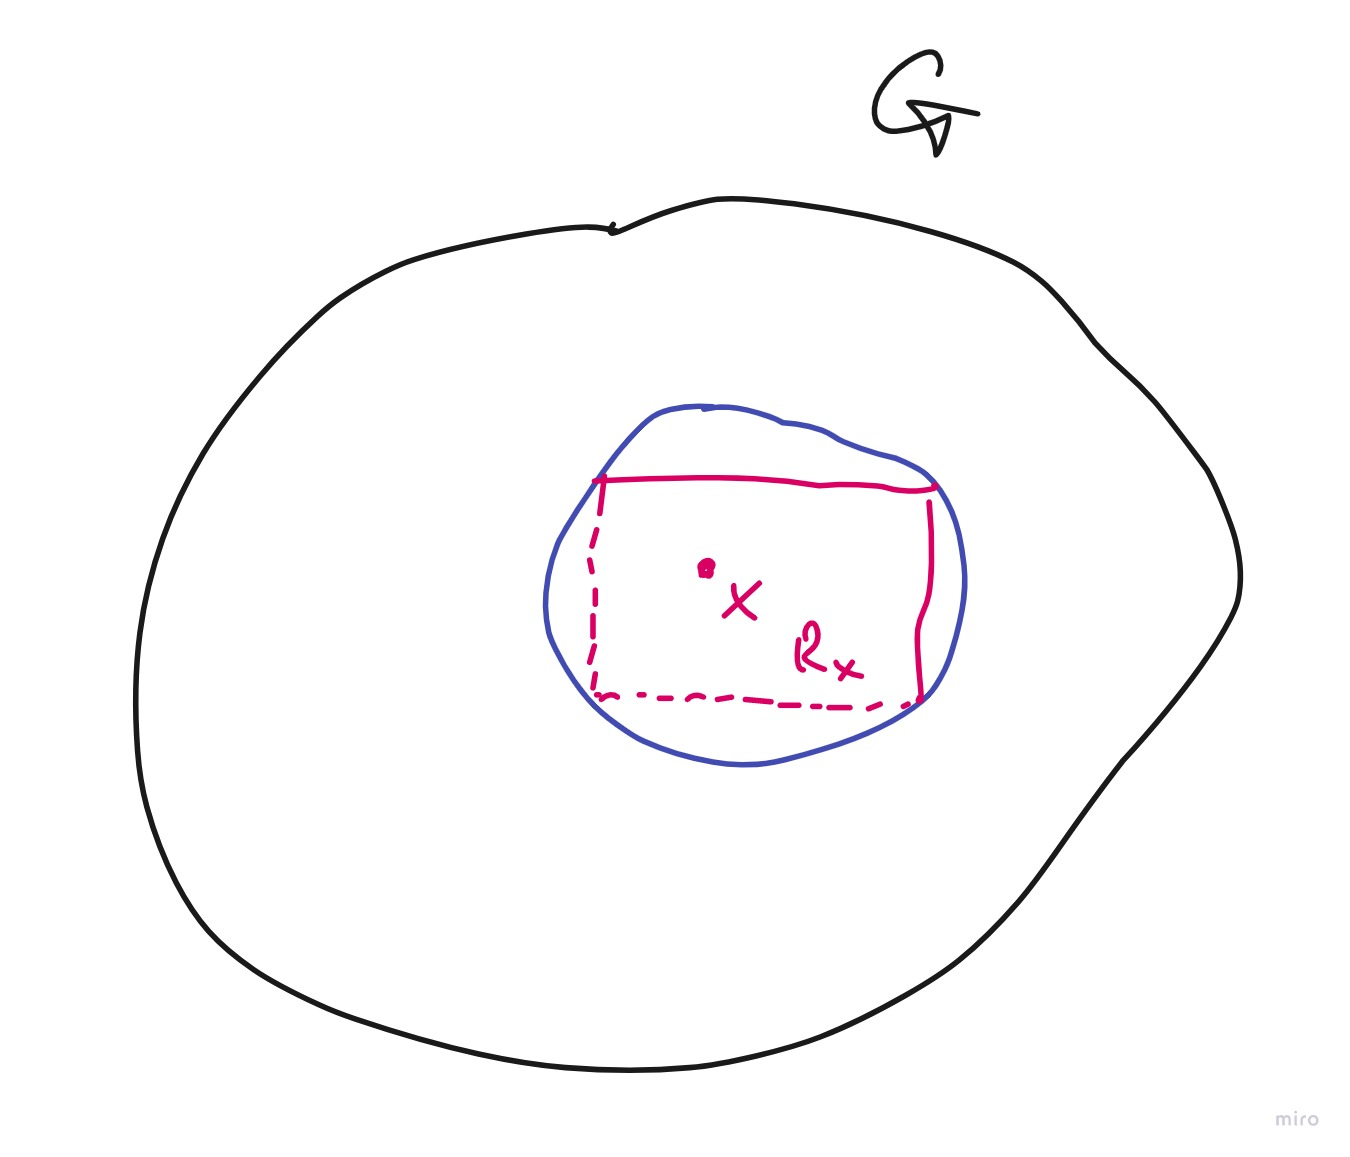
\includegraphics[scale=0.15]{./assets/01-measure-theory/opened-set-with-rect.jpg}
    }

    Выкинем повторы: $G = \bigcup_{n=1}^{\infty} R_{x_n} = \bigsqcup_{n=1}^{\infty} \bigsqcup_{j=1}^{m_n} Q_{nj}$
\end{proof}

\begin{consequence}
    $\mathcal{B}(\mathcal{P}^m_Q) = \mathcal{B}^m$.
\end{consequence}
\begin{proof}
    
    1. $\mathcal{P}^m \supset \mathcal{P}^m_Q \implies \mathcal{B}(\mathcal{P}^m) \supset \mathcal{B}(\mathcal{P}_Q^m)$

    $(a, b] \in \mathcal{B}^m \implies \mathcal{P}^m \subset \mathcal{B}^m \implies \mathcal{B}(\mathcal{P}^m) \subset \mathcal{B}^m$

    $G$ -- открытое $\implies G \in \mathcal{B}(\mathcal{P}_Q^m) \implies \mathcal{B}(\mathcal{P}^m_Q) \supset \mathcal{B}^m$
\end{proof}

\Subsection{Объем и мера}
\begin{definition}
    $\mathcal{P}$ -- полукольцо. $\mu: \mathcal{P} \rightarrow [0, +\infty]$. $\mu$ -- объем, если 

    \begin{enumerate}
        \item $\mu(\emptyset) = 0$
        \item Если $P_1, P_2, \dots, P_n \in \mathcal{P}$ и $\bigsqcup_{k=1}^n P_k \in \mathcal{P}$, то $\mu \left(\bigsqcup_{k=1}^n P_k\right) = \sum_{k=1}^{n} \mu P_k$ 
    \end{enumerate}
\end{definition}

\begin{definition}
    $\mu$ -- мера, если 

    \begin{enumerate}
        \item $\mu(\emptyset) = 0$
        \item Если $P_1, P_2, \dots \in \mathcal{P}$ и $\bigsqcup_{k=1}^{\infty} P_k \in \mathcal{P}$, то $\mu \underbrace{\left(\bigsqcup_{k=1}^{\infty} P_k\right)}_{\text{счетная аддитивность}} = \sum_{k=1}^{\infty} \mu P_k$ 
    \end{enumerate}
\end{definition}

\begin{exerc}
    $\mu$ -- мера. Если $\mu \not \equiv +\infty$, то условия $\mu \emptyset = 0$ выполнено автоматически.
\end{exerc}

\begin{example}
    \begin{enumerate}
        \item $\mathcal{P}^1$,   \;\; $\mu (a, b] := b - a$ -- длина (упр. доказать, что объем и мера).
        \item {
            $g: \mathcal{R} \rightarrow \mathcal{R}$ -- нестрого монотонная

            \begin{enumerate}
                \item $\mu_{g}(a, b] := g(b) - g(a)$ (упр. доказать, что объем).
            \end{enumerate}
        }
        \item $\mathcal{P}^m$ (m-мерные ячейки), \;\; $\mu (a, b] := (b_1 - a_1)(b_2 - a_2) \dots (b_m - a_m), \ a := (a_1, \ ..., \ a_m), \ b := (b_1, \ ..., \ b_m)$ -- классический объем.
        \item {
            $\mathcal{P} = 2^X$, \;\; $x_0 \in X$, \;\; $a \geq 0$
            
            \begin{equation}
                \mu A := 
                \begin{cases}
                    $a$, \ if \  x_{0} \in A \\
                    $0$, \ otherwise
                \end{cases}                
            \end{equation}

            $\mu$ - мера.
        }
        \item {
            $\mathcal{P}$ -- огр. мн-ва и их дополнения.
            
            \begin{equation}
                \mu A := 
                \begin{cases}
                    $1$, \ if \  x_{0} \in A \\
                    $0$, \ otherwise
                \end{cases}                
            \end{equation}

            $\mu$ - объем, но не мера.
        }
    \end{enumerate}
\end{example}

\begin{theorem}
    $\mu$ - объем на полукольце $\mathcal{P}$

    \begin{enumerate}
        \item Монотонность: $\mathcal{P} \ni P \subset \tilde{P} \in \mathcal{P} \implies \mu P \leq \mu \tilde{P}$
        \item {
            \begin{enumerate}
                \item Усиленная монотонность: $P_1, P_2, \dots P_n, P \in \mathcal{P}$. $\bigsqcup_{k=1}^n P_k \subset P \implies \sum_{k=1}^n \mu P_k \leq \mu P$
                \item Пункт (a), но $n = \infty$
            \end{enumerate}
        }
        \item Полуаддитивность: $P, P_1, P_2, \dots P_n \in \mathcal{P}$ и $P \subset \bigcup_{k=1}^{n}P_k$, тогда $\mu P \leq \sum_{k=1}^{n} \mu P_k$ 
    \end{enumerate}
\end{theorem}

\begin{proof}
    \begin{enumerate}
        \item Очев типо.
        \item {
        \begin{enumerate}
            \item $P \setminus \bigsqcup_{k=1}^{n} \mu P_k =  \bigsqcup_{j=1}^{m} Q_j \implies P = \bigsqcup_{k=1}^{n} P_k \sqcup \bigsqcup_{j=1}^m Q_j \implies \mu P = \sum_{k=1}^{n} \mu P_k + \sum_{j=1}^{m} \mu Q_j \geq \sum_{k=1}^{n} \mu P_k $
            \item $\bigsqcup_{k=1}^{\infty} P_k \subset P \implies \bigsqcup_{k=1}^n P_k \subset P \implies \sum_{k=1}^{n} \mu P_k \rightarrow \sum_{k=1}^{\infty} \mu P_k \leq \mu P$
        \end{enumerate}
        \item {
            $P_k' := P \cap P_k \in \mathcal{P}$ ($\mathcal{P}$ - полукольцо), \;\; $P = \bigcup_{k=1}^{n} P_k' = \bigsqcup_{k=1}^{n} \underbrace{\bigsqcup_{j=1}^{m_k} Q_{kj}}_{\in P_k'} \implies$
            
            $\implies \mu P = \sum_{k=1}^n \underbrace{\sum_{j=1}^{m_k} \mu Q_{kj}}_{\leq \mu P'_k \leq \mu P_k \ (property \ 2(a). )} \leq \sum_{k=1}^n \mu P_k$
        }
        }
    \end{enumerate}
\end{proof}

\begin{remark}
    \begin{enumerate}
        \item {
            Если $\mathcal{P}$ -- кольцо и $A, B$ ($B \subset A$) $ \in \mathcal{P}$, то $A \setminus B \in \mathcal{P}$

            $\mu (A \setminus B) + \mu B = \mu A$

            Если $\mu B \neq +\infty$, то $\mu (A \setminus B) = \mu A - \mu B$
        }
    \end{enumerate}
\end{remark}

\begin{theorem}
    $\mathcal{P}$ -- полукольцо подмн-в $X$, \mu -- объем на $\mathcal{P}$

    $\mathcal{Q}$ -- полукольцо подмн-в $Y$, \nu -- объем на $\mathcal{Q}$

    $\lambda(P \times Q) := \mu P \cdot \nu Q$, где $0 \cdot +\infty = +\infty \cdot 0 = 0$

    Тогда $\lambda$ -- объем на $P \times Q$.
\end{theorem}
\begin{consequence}
    Классический объем на ячейках -- действительно объем.
\end{consequence}
\begin{proof}
    Простой случай. $P = \bigsqcup_{k=1}^{n}P_k, Q = \bigsqcup_{j=1}^m Q_j$, тогда:

    $P \times Q = \bigsqcup_{k=1}^{n} \bigsqcup_{j=1}^{m} P_k \times Q_j$, докажем, что $\underbrace{\lambda (P \times Q)}_{\sum_{k=1}^n \mu P_k \cdot \sum_{j=1}^m \nu Q_j = \mu P \cdot \nu Q} = \sum_{k=1}^n \sum_{j=1}^m \underbrace{\lambda (P_k \times Q_j)}_{\mu P_k \cdot \nu Q_j}$

    Общий случай.

    \begin{center}
        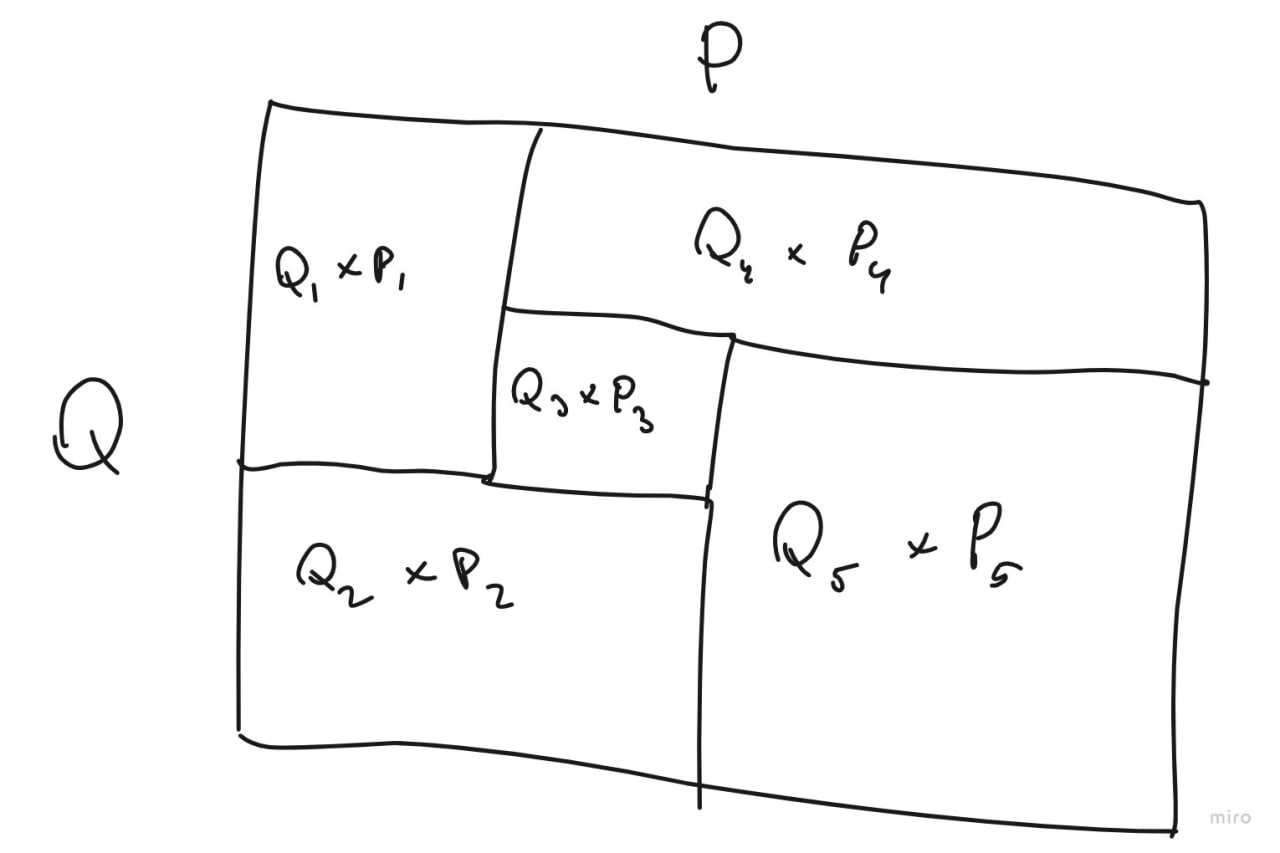
\includegraphics[scale=0.3]{./assets/01-measure-theory/PxQ.jpg}
    \end{center}

    $P \times Q = \bigsqcup_{k=1}^{n} P_k \times Q_k$
    
    $P = \bigcup_{k=1}^{n} P_k = \bigsqcup_{k=1}^{N} P_k'$

    $Q = \bigcup_{j=1}^{m} Q_j = \bigsqcup_{j=1}^{M} Q_j'$
\end{proof}

\begin{example}
    \begin{enumerate}
        \item Классический объем на ячейках $\lambda_m$ -- мера
        \item {
            $g : \mathbb{R} \rightarrow \mathbb{R}$ нестрого монотонная возрастающая и непрерывна слева во всех точках, тогда $\nu_g (a, b]:=g(b) - g(a)$ -- мера.

            (\underline{Rem}: $lim_{x \rightarrow a-} f(x) = f(a)$ -- непрерывность слева).
        }
        \item Считающаяся мера: $\mu A := \#A$ -- кол-во элементов.
        \item $T = \{t_1, t_2, \dots \}$ -- не более чем счетное множетсво, $w_1, w_2, \dots \geq 0$, $\mu A := \sum_{k: t_k \in A} w_k$ $\rightarrow$ $\mu$ -- мера.
    \end{enumerate}
\end{example}

\begin{proof}
    4. $A = \bigsqcup_{n=1}^{\infty} A_n \implies \mu A = \sum_{n=1}^{\infty} \mu A_n$

    Обозначения:

    \begin{enumerate}
        \item $\sum_{n=1}^{N} \sum_{k: \ t_k \in A_n} w_k \ (*)$.
        \item $\sum_{k: \ t_k \in A} w_k \ (**)$.
        \item $\sum_{n=1}^{\infty} \sum_{k: \ t_k \in A_n} w_k \ (***)$.
    \end{enumerate}

    \begin{enumerate}
        \item {
            $\mu A = \sum_{k: \ t_k \in A} w_k \ (**) \geq \sum_{n=1}^{N} \sum_{k: \ t_k \in A_n} w_k \ (*)$ -- т.к. $A_i \cap A_j = \emptyset \ (\forall i, \ j: \ i \neq j)$, то каждое слагаемое $w_k$ не более $1$ раза попадет в $(*)$ и $A = \bigsqcup_{n=1}^{\infty} A_n$.
        }

        \item {
            $\sum_{n=1}^{\infty} \mu A_n = \sum_{n=1}^{\infty} \sum_{k: \ t_k \in A_n} w_k \ (***) \geq \sum_{k: \ t_k \in A}$ -- нер-во верно, так как мы можем к каждому $w_k$ из $(**)$ найти этот же $w_k$ в $(***)$. 
        }

        Итого имеем равенство:

        $(**) = (***): \ \sum_{k: \ t_k \in A} w_k = \sum_{n=1}^{\infty} \sum_{k: \ t_k \in A_n} w_k \implies \mu A = \sum_{n=1}^{\infty} \mu A_n$, чтд.

        (\underline{От автора}: если у кого-то лучше расписано данное док-во, сделайте, пожалуйста, PR).
    \end{enumerate}
\end{proof}

\begin{theorem}
    О счетной аддитивности меры $\mu$-объем на полукольце $\mathcal{P}$. Тогда $\mu$-мера $\Leftrightarrow$ если $P \subset \bigcup_{n=1}^{\infty}P_n \ P, P_n \in \mathcal{P}$, то $\mu \cdot P \leq \sum_{n=1}^{\infty}\mu \cdot P_n$ (счетная полуаддитивность). 
\end{theorem}
\begin{proof}
    "$\leftarrow$": Пусть $P=\bigsqcup_{n=1}^{\infty} P_n$, тогда нажо д-ть, что $\mu P = \sum_{n=1}^{\infty} \mu P_n$: для "$\leq$" -- счетная полуаддитивность, для "$\geq$" -- усиленная монот. объема.

    "$\rightarrow$": $P_n' := P \cap P_n \implies P = \bigcup_{n=1}^{\infty}P_n' \implies P = \bigsqcup_{n=1}^{\infty} \bigsqcup_{k=1}^{\infty} Q_{nk}, $ где $Q_{nk} \subset P_n' \implies \mu P = \sum_{n=1}^{\infty} \underbrace{\sum_{k=1}^{m_k} \mu Q_{nk}}_{\leq \mu P_n}$ -- усиленная монот. объема. $\bigsqcup_{k=1}^{m_k} Q_{nk} \subset P_n' \subset P_n$.
\end{proof}

\begin{consequence}
    Если $\mu$-мера на \sigma-алгебре, то счетное объединение мн-в ненулевой меры -- мн-во нулевой меры.
\end{consequence}
\begin{proof}
    $\mu A_n = 0 \implies \mu \left( \bigcup_{n=1}^{\infty} \right) \leq \sum_{n=1}^{\infty} \mu A_n = 0$.
\end{proof}

\begin{theorem}
    о непрерывности меры снизу.

    $\mu$-объем на \sigma-алгебре $\mathcal{A}$. Тогда \mu-мера $\Leftrightarrow$ если $\mathcal{A} \ni A_n \subset A_{n+1}$, то $\mu \left( \bigcup_{n=1}^{\infty} A_n \right) = \lim_{n \rightarrow \infty }{\mu A_n}$ -- непр. меры снизу. 
\end{theorem}
\begin{proof}
    "$\rightarrow$": $\mathcal{A} \ni B_n := A_n \setminus A_{n-1}, \ A_0 = \emptyset$.

    $B_n$ -- дизъюнктны: $\bigsqcup_{n=1}^{\infty} B_n = \bigcup_{n=1}^{\infty} A_n$.

    $\mu \left( \bigcup A_n \right) = \mu \bigsqcup B_n = \sum_{n=1}^{\infty}\mu B_n = \lim_{n \rightarrow \infty} \sum_{k=1}^{n} \mu B_k = \lim \mu A_n$.

    "$\leftarrow$": Пусть $C = \bigsqcup_{n=1}^{\infty} C_n$, надо д-ть, что $\mu C = \sum_{n=1}^{\infty} \mu C_n$.

    $A_n := \bigsqcup_{k=1}^{n} C_k, \ A_n \subset A_{n+1}, \ \bigcup_{n=1}^{\infty} A_n = \bigsqcup_{n=1}^{\infty} C_n$

    $\underbrace{\mu \left( \bigcup_{n=1}^{\infty} A_n\right)}_{= \mu \left( \bigsqcup_{n=1}^{\infty} C_n\right)} = \lim \mu A_n = \lim \mu \left( \bigsqcup_{k=1}^{n} C_k\right)  = \lim \sum_{k=1}^{n} \mu C_k = \sum_{n=1}^{\infty} \mu C_n$
\end{proof}

\begin{theorem}
    о непрерывности меры сверху.

    \mu -- объем на \sigma-алгебре $\mathcal{A}$ и $\mu X < +\infty$.

    Тогда равносильны: 
    \begin{enumerate}
        \item \mu -- мера
        \item если $A_n \supset A_{n+1}$, то $\mu \left(\bigcap_{n=1}^{\infty} A_n\right) = \lim \mu A_n$
        \item если $A_n \supset A_{n+1}$ и $\bigcap_{n=1}^{\infty} A_n = \emptyset$, то $\lim \mu A_n = 0$.
    \end{enumerate}
\end{theorem}

\begin{proof}
    (1) $\implies $ (2): $A_n \supset A_{n+1} \implies B_n := X \setminus A_n \subset X \setminus A_{n+1} =: B_{n+1}$. $\bigcup_{n=1}^{\infty} B_n = X \setminus \bigcap_{n=1}^{\infty} A_n$.

    $\implies \underbrace{\mu \left( \bigcup_{n=1}^{\infty} B_n \right)}_{\mu (X \setminus \bigcap_{n=1}^{\infty} A_n)} = \lim \mu B_n = \lim \mu (X \setminus A_n) = \lim (\mu X - \mu A_n)$


    (3) $\implies $ (1): $C = \bigsqcup_{n=1}^{\infty} C_n$, надо д-ть, что $\mu C = \sum_{n=1}^{\infty} \mu C_n$.

    $A_n := \bigsqcup_{k=n + 1}^{\infty} C_k, \ A_n \supset A_{n+1}$ и $\bigcap_{n=1}^{\infty} A_n = \emptyset$, тогда $\lim \mu A_n = 0$.

    $C = \bigsqcup_{k=1}^{n} C_k \sqcup A_n \implies \mu C  = \sum_{k=1}^{n} \mu C_k + \mu A_n$.
\end{proof}

\begin{consequence}
    Если \mu-- мера, то $A_n \supset A_{n+1}$ и  для некоторого $m \ \mu A_m < +\infty$
\end{consequence}
\begin{proof}
    $X := A_n$
\end{proof}
\begin{exerc}
    Придумать объем, не являющийся мерой, обладающей св-вом из следствия. 
\end{exerc}

\Subsection{Продолжение мер}
\begin{definition}
    $\nu : 2^{X} \rightarrow [0; +\infty]$ -- субмера, если 

    \begin{enumerate}
        \item $\nu \emptyset = 0$
        \item монотонность: если $A \subset B$, $\nu A \leq \nu B$
        \item счетная полуаддитивность: если  $A \subset \bigcup_{n=1}^{\infty} A_n$, то $\nu A \leq \sum_{n=1}^{\infty} \nu A_n$
    \end{enumerate}
\end{definition}
\begin{remark}
    \begin{enumerate}
        \item счетная полуаддитивность $\implies$ конечная.
        \item монотонность (следует из счетной полуаддитивности) $A \subset B, \ n=1$.
    \end{enumerate}
\end{remark}

\begin{definition}
    \mu -- полная мера на \sigma-алгебре $\mathcal{A}$, если $A \subset B \in \mathcal{A}$ и $\mu B = 0 \implies A \in \mathcal{A}$.
    
    \begin{remark}
        это означает, что $\mu A = 0$.
    \end{remark}
\end{definition}
% TODO: выше нужно пофиксить места, где вместо $\implies$ влево и вправо написаны $\rightarrow / \leftarrow$ в доказательсвах, разбитых на стрелки вправо/влево

\begin{definition}
    $\nu$ -- субмера, назовем $E \subset X \ \nu$-измеримым, если $\forall A \subset X \ \nu A = \nu (A \cap E) + \nu (A \setminus E)$

    % TODO: picture

    \begin{remark}
        Достаточен знак "$\geq$" (следует из счетной полуаддитивности).
    \end{remark}
\end{definition}

\begin{theorem}
    \textbf{Каратеодори}. Пусть \nu -- субмера. Тогда $\nu$-измеримое мн-во образует \sigma-алгебру и сужение \nu на эту \sigma-алгебру -- полная мера.
\end{theorem}

\begin{proof}
    Обозначим через $\mathcal{A} \ \nu$-измеримые мн-ва. 

    \begin{enumerate}
        \item {
            Если $E = 0$, то $E \in \mathcal{A}$. 

            $\forall A \subset X, \ \nu A \underbrace{\geq}_{?} \nu (A \cap E) + \nu (A \setminus E)$

            $A \cap E \subset E, \ \nu (A \cap E) \leq \nu E = 0 \implies \nu (A \cap E) = 0$, тогда доказали вопросик сверху. 
        }
        \item {
            $\mathcal{A}$ -- симметричное семейство мн-в.
            
            $E \in \mathcal{A} \implies X \setminus E \in \mathcal{A}$
            
            $A \cap E = A \setminus (X \setminus X)$

            $A \setminus E = A \cap (X \setminus E)$
        }
        \item {
            Если $E$ и $F \in \mathcal{A}$, то $E \cup F \in \mathcal{A}$
            
            $\nu A = \nu (A \cap E) + \nu (A \setminus E) = \underbrace{\nu (A \cap E) + \nu ((A \setminus E) \cap F)}_{\geq \nu (A \cap (E \cup F))} + \underbrace{\nu ((A \setminus E) \setminus F)}_{\nu (A \setminus (E \cup F))} \geq \nu (A \cap (E \cup F)) + \nu (A \setminus (E \cup F))$
            % TODO: picture
        }
        \item $\mathcal{A}$ -- алгебра.
        \item {
            $E = \bigsqcup_{n=1}^{\infty}E_n$, где $E_n \in \mathcal{A} \underbrace{\implies}_{?} E \in \mathcal{A}$.

            $\nu A = \nu (A \cap \bigsqcup_{k=1}^{n} E_k) + \nu (A \setminus \bigsqcup_{k=1}^{n} E_k) \geq \underbrace{\nu (A \cap \bigsqcup_{k=1}^{n} E_k)}_{\nu (A \cap E_n) + \nu (A \cap \bigsqcup_{k=1}^{n-1}E_k)} + \nu (A \setminus E) \implies$
            
            $\implies \nu A \geq \underbrace{\sum_{k=1}^{\infty} \nu (A \cap E_k)}_{\geq \nu (\bigcup_{k=1}^{\infty} (A \cap E_k)) = \nu (A \cap E)} + \nu (A \setminus E) \geq \nu (A \cap E) + \nu (A \setminus E)$.

            % TODO: picture
        }
        \item Если $E_n \in \mathcal{A}$ и $E = \bigcup_{n=1}^{\infty}$, то $E \in \mathcal{A}$.
        \item $\mathcal{A}$ -- \sigma-алгебра.
        \item {
            \nu -- мера на $\mathcal{A}$.

            $E = \bigsqcup_{n=1}^{\infty} E_n \underbrace{\implies}_{?} \nu E = \sum_{n=1}^{\infty} \nu E_n$ ($leq$ уже есть).

            Докажем, что $\nu E \geq \sum_{k=1}^{n} \nu E_k$. Знаем, что $\nu E \geq \nu (\bigsqcup_{k=1}^{n} E_k) = \sum_{k=1}^{n} \nu E_k$
        }
    \end{enumerate}
\end{proof}

\begin{definition}
    \mu -- мера на полукольце $\mathcal{P}$, $A \subset X$.

    $\mu^* A := \inf{ \left\{\sum_{k=1}^{\infty} \mu P_k: \ P_k \in \mathcal{P} \ \land \ A \subset \bigcup_{k=1}^{\infty} P_k \right\}}$

    если покрытия нет, то $+\infty$.

    -- внешняя мера, порожд. $\mu$.
\end{definition}
\begin{remark}
    \begin{enumerate}
        \item {
            Можно считать, что $P_k$ -- дизъюнктны

            $A \subset \bigcup_{n=1}^{\infty} P_n = \bigsqcup_{n=1}^{\infty} \bigsqcup_{k=1}^{m_k} Q_{nk}, \ \sum_{n=1}^{\infty} \sum_{k=1}^{n=m_k} \mu Q_{nk} \leq \sum_{n=1}^{\infty} \mu P_n$
        }
        \item {
            Если $\mu$ задана на \sigma-алгебре $\mathcal{A}$, то $\mu^* A = \inf \left\{\mu B \ : \ B \in \mathcal{A} \ \land \ A \subset B \right\}$
        }
    \end{enumerate}
\end{remark}

% TODO: добавить '$...$' вокруг греческих букв, записанных без доллара, так как возникает проблема, что пробелы после таких букв удаляются и буквы сливаются со словами воедино.

\begin{theorem}
    Пусть $\mu$ -- мера на полукольце $\mathcal{P}$. Тогда $\mu^*$ -- субмера, совпадающая с мерой $\mu$ на полукольце $\mathcal{P}$.
\end{theorem}
\begin{proof}
    \begin{enumerate}
        \item {
            $A \in \mathcal{P}$, хотим доказать, что $\mu A = \mu^* A$.

            "$\geq$": очевидно, так как множество покрывает само себя. $\mu^* A = \inf\left\{ \sum_{k=1}^{\infty} \mu P_k \ : \ \bigcup_{k=1}^{\infty} P_k \supset A \right\}$

            "$\leq$": $S \subset \bigcup_{k=1}^{\infty} P_k \underbrace{\implies}_{\text{счетная полуаддитивность}} \mu A_n \leq \sum_{k=1}^{\infty} \mu P_k \implies \mu A \leq \inf = \mu^* A$
        }
        \item {
            $\mu^*$ -- субмера, т.е. нужна счетная полуаддитивность.

            $A \subset \bigcup_{n=1}^{\infty} A_n \underbrace{\implies}_{?} \mu^* A \leq \sum_{n=1}^{\infty} \mu^* A + \epsilon$

            $\mu^* A_n = \inf ... $, берем покрытие $A_n \subset \bigcup_{k=1}^{\infty} P_{nk}$ т.ч. $\sum_{k=1}^{\infty} \mu P_{nk} < \mu^* A_n + \frac{\epsilon}{2^n}$

            $\mu^* A \leq \sum_{n=1}^{\infty} \sum_{k=1}^{\infty} \mu P_{nk} < \sum_{n=1}^{\infty} \mu^* A_n + \epsilon$ и $A \subset \bigcup_{n=1}^{\infty} A_n \subset \bigcup_{n=1}^{\infty} \bigcup_{k=1}^{\infty} P_{nk}$ -- устремляем $\epsilon$ к нулю.

        }
    \end{enumerate}
\end{proof}

\begin{definition}
    Стандартное продолэение меры $\mu_0$ с полукольца $\mathcal{P}$. $\mu^*_0$ -- внешняя мера, порождающая $\mu_0$ -- субмера, и сужаем ее на все $\mu^*_0$ -- измеримые мн-ва.

    Получилась полная мера $\mu$ на \sigma-алгебра $\mathcal{A} \supset \mathcal{P}$ и $\mu P = \mu_0 P$ для $P \in \mathcal{P}$.

    Обозначение мн-ва из $\mathcal{A}$ назовем $\mu$-измеримыми.
\end{definition}

\begin{theorem}
    Это действительно продолжение, то есть $\mathcal{A} \supset \mathcal{P}$.
\end{theorem}
\begin{proof}
    Надо доказать, что $E \in \mathcal{P} \ \land \ A \subset X$, $\mu^*_0 A \geq \mu^*_0 (A \setminus E) + \mu^*_0 (A \cap E)$.

    Рассмотрим случаи:
    \begin{enumerate}
        \item {
            $A \in \mathcal{P}$.

            $\mu^*_0 A = \mu_0 A, \ \mu^*_0 (A \cap E) = \mu_0 (A \cap E)$

            $A \setminus E = \bigsqcup_{k=1}^{n} Q_k, \ Q_k \in \mathcal{P}$

            $A = (A \cap E) \sqcup \bigsqcup_{k=1}^{n} Q_k \implies \mu^*_0 A = \mu_0 A = \underbrace{\sum_{k=1}^{n} \mu_0 Q_k}_{\geq \mu^*_0 (A \setminus E)} + \underbrace{\mu_0 (A \cap E)}_{\mu^*_0 (A \cap E)}$
        }
        \item {
            $A \notin \mathcal{P}$.

            Если $\mu^*_0A = +\infty$, то все очевидно, поэтому считаем, что оно конечно.

            Считаем, что $\mu^*_0 A < +\infty$. Возьмем $P_k \in \mathcal{P}$, такое что $A \subset \bigcup_{k=1}^{\infty} P_k$ и $\sum_{k=1}^{\infty} \mu_0 P_k < \mu^*_0 A + \epsilon$.

            Знаем, что $\mu^*_0 P_k \geq \mu^*_0 (P_k \setminus E) + \mu^*_0 (P_k \cap E)$

            $\mu^*_0 A + \epsilon > \sum_{k=1}^{\infty} \mu_0 P_k \geq \underbrace{\sum_{k=1}^{\infty} \mu^*_0 (P_k \setminus E)}_{\geq \mu^*_0 (\bigcup_{k=1}^{\infty} (P_k \setminus E)) \geq \mu^*_0 (A \setminus E)} + \underbrace{\sum_{k=1}^{\infty} \mu^*_0 (P_k \cap E)}_{\geq \mu^*_0 (\bigcup_{k=1}^{\infty} (P_k \cap E)) \geq \mu^*_0 (A \cap E)}$
        }
    \end{enumerate}
\end{proof}

\begin{remark}
    \begin{enumerate}
        \item {
            Дальше мера и ее продолжение обозначаем как $\mu$.

            Если $A$ -- $\mu$-измеримое множество, то $\mu A = \inf \left\{ \sum_{k=1}^{\infty} \mu P_k \ : \ A \subset \bigcup_{k=1}^{\infty} P_k \ \land \ P_k \in \mathcal{P} \right\}$
        }
        \item {
            Стандартное продолжение, примененое к стандартному продолжению, не дает ничего нового.

            \begin{exerc}
                Указание. Проверить, что стандартное продолжение порождает ту же врешнюю меру, что и $\mu$.
            \end{exerc}
        }
        \item {
            Можно ли распространить меру на более широкую \sigma-алгебру.
        }
        \item {
            \begin{definition}
                $\nu$ -- \sigma-конечная мера на полукольце $\mathcal{P}$, если $X = \bigcup_{n=1}^{\infty}P_n, \ P_n \in \mathcal{P} \ \land \ \mu P_n < +\infty$.
            \end{definition}
            
            Можно ли по-другому продолжить на \sigma-алгебру \mu-измерим. мн-в?

            Если $\mu$ -- $\sigma$-конечная мера, то нельзя.
        }
        \item {
            Обязательно ли полная мера будет задана на $\mu$-измеримых множествах.

            Если $\mu$ -- $\sigma$-конечная мера, то обязательно.
        }
    \end{enumerate}
\end{remark}


\begin{theorem}
    $\mu$-стандартное продолжение меры с полукольца $\mathcal{P}$. $\mu^*$ -- соответствующая внешняя мера, $A \subset X$, $\mu^* A < + \infty$. Тогда $\exists B_{nk} \in \mathcal{P}$, такие что $C_{n} := \bigcup_{k=1}^{\infty} B_{nk}, \ C := \bigcap_{n=1}^{\infty} C_n$, $C \supset A \ \land \ \mu^* A = \mu C$.
\end{theorem}
\begin{proof}
    $\mu^* A = \inf \left\{ \sum_{k=1}^{\infty} \mu P_k \ : \ A \subset \bigcup_{k=1}^{\infty} P_k \ \land \ P_k \in \mathcal{P} \right\}$, берем покрытие с суммой $< \mu^* A + \frac{1}{n}$.

    $\mu C_n \leq \sum_{k=1}^{\infty} \mu B_{nk} < \mu^* A + \frac{1}{n}, \ C_n = \bigcup_{k=1}^{\infty} B_{nk} \supset A \implies C = \bigcap_{n=1}^{\infty} C_n \supset A$.

    $\mu^*A \leq (\mu^* C = \mu C) \leq \mu C_n < \mu^* A + \frac{1}{n}$
\end{proof}

\begin{consequence}
    $\mu$-стандартное продолжение с полукольца $\mathcal{P}$. $A$ -- $\mu$-измеримое мн-во и $\mu A < +\infty$. Тогда $A = B \sqcup e$, где $B \in \mathcal{B}(\mathcal{P})$ и $\mu e = 0$.
\end{consequence}
\begin{proof}
    Берем $C \underbrace{\in \mathcal{B}(\mathcal{P})}_{\text{получаем автоматически}}$ из теоремы. $A \subset C$, и $\mu A = \mu C$.

    $e_1 := C \setminus A, \ \mu e_1 = 0$, теперь подставляем $e_1$ в теорему: 
    
    найдется $e_2: \ e_2 \in \mathcal{B}(\mathcal{P}) \ \land  \ e_2 \supset e_1 \ \land \ \mu e_2 = \mu e_1 = 0 \implies B := C \setminus e_2 \in \mathcal{B}(\mathcal{P}) \implies B \subset A$.

    $C \setminus e_2 \subset B \subset C$, $\mu C = \mu C - \mu e_2 \leq \nu B \leq \mu C \implies \mu B = \mu A$. $e = A \setminus B \implies \mu e = 0$

    % TODO: picture
\end{proof}

\begin{theorem}
    Единственность продолжения $\mu$-стандартное продолжение с полукольца $\mathcal{P}$ на $\sigma$-алгебру $\mathcal{A}$.

    $\nu$ -- другая мера на $\mathcal{A}$, совпадающая с $\mu$ на $\mathcal{P}$. Если $\mu$ -- $\sigma$-конечная, то $\mu = \nu$.
\end{theorem}

\begin{proof}
    Если $A \subset \bigcup_{n=1}^{\infty} P_n, \ P_n \in \mathcal{P},$ то $\sum_{n=1}^{\infty} \mu P_n = \sum_{n=1}^{\infty} \nu P_n \geq \nu A$ (пользуемся счетной полуаддитивностью).

    $\mu A = \inf \left\{ \sum \mu P_n \right\} \geq \nu A$.

    Возьмем $P \in \mathcal{P}$, $A \in \mathcal{A}$: $\mu P = \nu P \implies \nu (P \cap A) + \nu (P \setminus A) \leq \mu (P \cap A) + \mu (P \setminus A) = \mu P$

    Если $\mu P < + \infty$, то равенство вместо неравенства.

    $\implies \mu (P \cap A) = \nu (P \cap A)$

    $X = \bigsqcup_{k=1}^{\infty} P_k$, т.ч. $\mu P_k < +\infty \implies \mu (P_k \cap A) = \nu (P_k \cap A)$

    $\mu A = \sum_{k=1}^{\infty} \mu (P_k \cap A) = \sum_{k=1}^{\infty} \nu (P_k \cap A) = \nu A$
\end{proof}


\Subsection{Мера Лебега}

\begin{theorem}
    Классический объем $\lambda_m$ на полукольце ячеек $\mathcal{P}^m$ -- мера.
\end{theorem}

\begin{proof}
    $(a; b] = \bigsqcup_{k=1}^{\infty} (a_k; b_k] \underbrace{\implies}_{?} \lambda (a; b] \leq \sum_{k=1}^{\infty} \lambda (a_k; b_k]$.

    $(a; b] \supset [a'; b] \supset (a'; b]$, т.ч. $\lambda (a; b] < \lambda(a'; b] + \epsilon$.

    $(a_k; b_k] \subset (a_k; b_k') \subset (a_k; b_k'], \ \lambda (a_k; b_k'] < \lambda (a_k; b_k] + \frac{\epsilon}{2^k}$

    компакт -- $[a'; b] \subset \bigcup_{k=1}^{\infty} (a_k; b_k')$, выбираем конечное подпокрытие.

    % TODO: picture

    $(a', b] \subset [a', b] \subset \sum_{k=1}^{n} (a_k; b_k') \subset \bigcup_{k=1}^{n} (a_k; b_k']$.

    $\lambda$ -- объем $\implies$ конечная полуаддитивность
    
    $\lambda (a'; b] \leq \sum_{k=1}^{n} \lambda (a_k; b_k'] < \sum_{k=1}^{n} (\lambda (a_k; b_k] + \frac{\epsilon}{2^k}) < \sum_{k=1}^{\infty} (\lambda [a_k; b_k] + \frac{\epsilon}{2^k})$

    % TODO: тут немного не успел, поправьте.
\end{proof}

\begin{definition}
    Мера Лебега в $\mathbb{R}^n$ (обозначение $\lambda_m$) -- стандартное продолжение классического объема с $\mathcal{P}^m$.

    $\sigma$-алгебра, на которую все продолжилось, лебегевская $\sigma$-алгебра $(\mathcal{X}^m)$. 
\end{definition}
\begin{remark}
    $\lambda_m A = \inf \{ \sum_{k=1}^{\infty} \lambda_m P_k \ : \ P_k - \text{ ячейки и } \bigcup_{k=1}^{\infty} P_k \supset A \}$.

    Можно вместо $P_k \in \mathcal{P}^m$ писать $P_k \in \mathcal{P}_Q^m$.
\end{remark}

\begin{properties}
    Свойства меры Лебега:

    \begin{enumerate}
        \item {
            Открытое мн-во измеримо и мера непустого открытого > 0.

            \begin{proof}
                Пусть $G$ - открытое, $x \in G$, $B$ -- шар, накрывающий $x$ и $B \subset G$, вписываем ячейку в шар.
                %  todo: picture
            \end{proof}
        }
        \item {
            Замкнутое мн-во измеримо и мера одноточечного мн-ва = 0.

            \begin{proof}
                Берем точку и ячейку, которая ее накрывает (стороны по $\epsilon$), тогда $\lambda_m E_{\epsilon} = \epsilon^m \implies \inf = 0$.
                % todo: small picture
            \end{proof}
        }
        \item {
            Мера ограниченного мн-ва конечна.

            \begin{proof}
                Есть множество, его можно положить в шар, а шар в кубик.

                % todo: picture
            \end{proof}
        }
        \item {
            Всякое измеримое мн-во -- объединение мн-в конечной меры.

            \begin{proof}
                Берем все $\mathbb{R}^m$ и нарежем его на ячейки по целочисленной сетке, тогда $\mathbb{R}^m = \bigsqcup_{k=1}^{\infty} \underbrace{P_k}_{\text{ячейки по сетке $\mathbb{Z}$}}$, тогда $E = \bigsqcup_{k=1}^{\infty}\underbrace{(P_k \cap E)}_{\text{ограничено и измеримо}}$.
            \end{proof}
        }
        \item {
            Пусть $E \subset \mathbb{R}^m$, такое что $\forall \epsilon > 0: \ \exists A_{\epsilon}, B_{\epsilon} \in \mathcal{X}^m$.
            
            $A_{\epsilon} \subset E \subset B_{\epsilon}$ и $\lambda_m (B_{\epsilon} \setminus A_{\epsilon}) < \epsilon$, тогда $E \in \mathcal{X}^m$
            
            \begin{proof}
                % todo: picture

                $A := \bigcup_{n=1}^{\infty} A_{\frac{1}{n}} \in \mathcal{X}^m$ и $B := \bigcap_{n=1}^{\infty} B_{\frac{1}{n}} \in \mathcal{X}^m$.

                $A \subset E \subset B$, $B \setminus A \subset B_{\frac{1}{n}} \setminus A_{\frac{1}{n}}$.

                $\lambda_m (B \setminus A) \leq \lambda_m (B_{\frac{1}{n}} \setminus A_{\frac{1}{n}}) < \frac{1}{n} \implies \lambda_m (B \setminus A) = 0$.

                $E \setminus A \subset B \setminus A \implies E \setminus A \in \mathcal{X}^m \implies E = E \setminus A \sqcup A \in \mathcal{X}^m$.
            \end{proof}
        }
        \item {
            Пусть $E \subset \mathbb{R}^m$, такое что $\forall \epsilon > 0: \ \exists B_{\epsilon} \in \mathcal{X}^m$, такое что $\lambda_m B_{\epsilon} < \epsilon$ и $E \subset B_{\epsilon}$.

            Тогда  $E \in \mathcal{X}^m$ и $\lambda_m E = 0$.

            \begin{proof}
                $A_{\epsilon} := \emptyset \underbrace{\implies}_{\text{свойство (5)}}$ E -- измеримое.

                $\lambda E \leq \lambda B_{\epsilon} < \epsilon \implies \lambda E = 0$.
            \end{proof}
        }
        \item {
            Счетное объединение мн-в нулевой меры -- мн-во нулевой меры.
        }
        \item {
            Счетное мн-во имеет меру 0.
        }
        \item {
            Мн-во нулевой меры не имеет внутренних точек.

            \begin{proof}
                Пусть $x \in Int E \implies \underbrace{B_r(x)}_{\text{непустое и открытое}} \subset E \implies 0 < \lambda B_r(x) \leq \lambda E$.
            \end{proof}
        }
        \item {
            Если $\lambda e = 0$, то существуют кубические ячейки $Q_j$, такие что $\bigcup_{j=1}^{\infty}A_j \supset e$ и $\sum_{j=1}^{\infty} \lambda Q_j < \epsilon$.

            \begin{proof}
                $0 = \lambda_m e = \inf \{ \sum_{j=1}^{\infty} \lambda P_j : \ P_j \in \mathcal{P}_{\mathbb{Q}^m} \ \land \ \bigcup_{j=1}^{\infty}P_j \supset e \}$, нарезаем $P_j$ на кубические ячейки.
            \end{proof}
        }
        \item {
            Если $m \geq 2$, то гиперплоскость $H_k(c) := \{ x \in \mathbb{R}^m : \ x_k = c \}$ имеет нулевую меру.

            \begin{proof}
                $E_n := H_k(c) \cap (-n, n]^m$, $H_k(c) = \bigcup_{n=1}^{\infty} E_n$. Достаточно доказать, что $\lambda E_n = 0$. $E_n \subset Y := (-n, n] \times \dots (-n, n] \times (c - \epsilon, c] \times (-n, n] \times \dots$.
                
                $\lambda E_n \leq \lambda Y = (2 n)^{m - 1} \cdot \epsilon$, так как $n$ фиксированное, а $\epsilon$ -- произвольное $\implies \lambda E_n = 0$.
            \end{proof}

            Любое мн-во, содержащееся в не более чем счетном объединение таких гиперплоскостей, имеет нулевую меру.
        }
        \item {
            $\lambda (a, b] = \lambda [a, b] = \lambda (a, b)$ -- по предыдущему свойству.
            % picture
        }
    \end{enumerate}
\end{properties}

\begin{remark}
    Свойства (5) и (6) -- справедливы для любой полной меры.
\end{remark}

\begin{remark}
    \begin{enumerate}
        \item {
            Существуют несчетные множества нулевой меры.
            
            Если $m \geq 2$, то пример это гиперплоскость $H_1 (c)$ подходит.

            Если $m = 1$, то подходит \href{https://ru.wikipedia.org/wiki/%D0%9A%D0%B0%D0%BD%D1%82%D0%BE%D1%80%D0%BE%D0%B2%D0%BE_%D0%BC%D0%BD%D0%BE%D0%B6%D0%B5%D1%81%D1%82%D0%B2%D0%BE}{Канторого множество}.

            $\lambda K = \underbrace{\lambda [0, 1] - \sum_{k=1}^{\infty} \lambda I_k}_{1 - \frac{1}{3} - 2 \cdot \frac{1}{9} - 4 \cdot \frac{1}{27} \dots = 1 - \sum_{k=1}^{\infty}\frac{2^{k-1}}{3^k} = 1 - \frac{1}{3} \cdot \frac{1}{1 - \frac{2}{3}} = 0 }$

            $K$ -- несчетно, $K = \{ x \in [0, 1]: \text{ в троичной записи нет цифр 1} \}$, а у таких чисел есть биекция между $[0, 1]$, просто троичную переводим в двоичную, где просто все двойки заменяем на единички.
        }
        \item {
            Существует неизмеримые мн-ва. Более того, любое мн-во положительной меры содержит неизмеримые подмножества.
        }
    \end{enumerate}
\end{remark}

\begin{theorem}
    (регулярность меры Лебега). Если $E$ -- измеримое, то найдется $G$ -- открытое, такое что оно накрывает $E$ и мера зазора $< \epsilon$, то есть $E \subset G \ \land \ \lambda (G \setminus E < \epsilon)$.
\end{theorem}
\begin{proof}
    $\lambda E = \inf \{ \sum_{j=1}^{\infty} \lambda P_j : \ P_j \text{ -- ячейка и } E \subset \bigcup_{j=1}^{\infty} P_j \}$.

    (1): Пусть $\lambda E < + \infty$. Возьмем покртыие, для которого $\sum \lambda P_j < \lambda E + \epsilon$.

    $(a_j, b_j] \subset (a_j, b_j')$, хотим $\lambda (a_j, b_j') < \lambda(a_j, b_j] + \frac{\epsilon}{2^j}$.

    Тогда $G := \bigcup_{j=1}^{\infty} (a_j, b_j')$ -- открытое и $E \subset G$.

    $\lambda G \leq \sum_{j=1}^{\infty} \lambda (a_j, b_j') < \sum_{j=1}^{\infty} \left( \lambda (a_j, b_j] + \frac{\epsilon}{2^j} \right) = \epsilon + \sum_{j=1}^{\infty} \lambda (a_j, b_j] < \lambda E + 2 \epsilon \implies \lambda (G \setminus E) < 2 \epsilon$


    (2): Пусть $\lambda E = +\infty$. $E = \bigsqcup_{n=1}^{\infty} E_n$, такие что $\lambda E_n < +\infty$. 

    Возьмем $G_n$ -- открытое $\supset E_n$, такое что $\lambda (G_n \setminus E_n) < \frac{\epsilon}{2^n}$.
    
    $G:=\bigcup_{n=1}^{\infty} G_n$ -- открытое $G \supset E$.

    $G \setminus E \subset \bigcup_{n=1}^{\infty} G_n \setminus E_n \implies \lambda (G \setminus E) \leq \sum \lambda (G_n \setminus E_n) < \underbrace{\sum \frac{\epsilon}{2^n}}_{= \epsilon}$.
\end{proof}

\begin{consequence}
    \begin{enumerate}
        \item {
            Если $E$ -- измеримо, то найдется $F \subset E$ -- замкнутое, такое что $\lambda (E \setminus F) < \epsilon$.

            \begin{proof}
                $G \supset \mathbb{R}^m \setminus E$, такое что $\lambda \underbrace{(G \setminus (\mathbb{R}^m \setminus E))}_{= E \setminus (\mathbb{R}^m \setminus G) = E \setminus F} < \epsilon$, где $F := \mathbb{R}^m \setminus G$ -- замкнутое и $F \subset E$.
            \end{proof}
        }
        \item {
            Если $E$ -- измеримо, то
            
            $\lambda E = \inf \{ \lambda G : \ G \text{ -- открытое и } G \supset E \}$.

            $\lambda E = \sup \{ \lambda F : \ F \text{ -- замкнуто и } F \subset E \}$
            
            $\lambda E = \sup \{ \lambda K : \ K \text{ -- компакт и } K \subset E \}$
            
            \begin{proof}
                
                $\lambda (G \setminus E) < \epsilon \implies \lambda E \leq \lambda G < \lambda E + \epsilon$


                $\lambda (E \setminus F) < \epsilon \implies \lambda E \geq \lambda F > \lambda E - \epsilon$

                Возьмем $F$ -- замкнутое из второго вывода и $K_n := [-n, n]^m \cap F$ -- компакт. $\bigcup_{n=1}^{\infty} K_n = F$ и $K_n \subset K_{n+1} \implies \lambda F = \lim{\lambda K_n}$

                Если $\lambda F = +\infty$, то есть $K_n$ со сколь угодно большой мерой.

                Если $\lambda F < +\infty$, то есть $K_n$, такие что $\lambda F < \lambda K_n + \epsilon$
            \end{proof}
        }
        \item {
            Если $E$ -- измеримо, то сузествует последовательность компактов $K_n$, такая что компакты $K_n \subset K_{n+1}$ и $E = \bigcup_{n=1}^{\infty} K_n \cup e$, где $\lambda e = 0$.

            \begin{proof}
                (1) Пусть $\lambda E < +\infty$. Возьмем $\tilde{K_n} \subset E \ \land \ \lambda E < \lambda \tilde{K_n} + \frac{1}{n}$

                $K_n := \bigcup_{j=1}^{n} \tilde{K_j} \subset E$, $\lambda E < \lambda \tilde{K_n} + \frac{1}{n} \leq \lambda K_n + \frac{1}{n}$.

                $e := E \setminus \bigcup_{n=1}^{\infty} K_n$, $\lambda e = \lambda E - \lambda \left( \bigcup_{n=1}^{\infty} K_n \right) < \lambda E - \lambda K_n < \frac{1}{n} \implies \lambda e = 0$.

                (2) Пусть $\lambda E = +\infty$. Берем $E = \bigsqcup_{j=1}^{\infty} E_j: \ \lambda E_j < +\infty$.

                $E_j = \bigcup_{n=1}^{\infty} \underbrace{K_{jn}}_{\text{компакт}} \cup e_j$ ($\lambda e_j = 0$) $\implies E = \bigcup_{j=1}^{\infty} \bigcup_{n=1}^{\infty} K_{jn} \cup e$, где $e = \bigcup_{j=1}^{\infty} e_j \ \land \ \lambda e = 0$.

                Нам не хватает вложенности, давайте просто пообъединяем их и получим новые компакты (вроде так, поправьте, если нет).
            \end{proof}
        }
    \end{enumerate}
\end{consequence}

\begin{exerc}
    $E$ -- измеримое. Д-ть, что $\exists G_n$ -- открытое $\supset E, \ G_n \supset G_{n+1}$, т.ч. $E = \bigcap_{n=1}^{\infty} G_n \setminus e$, где $\lambda e = 0$. 
\end{exerc}

\begin{theorem}
    При сдвиге мн-ва на верктор $\vec{v}$ измеримость сохраняется и мера не изменяется.
\end{theorem}
\begin{proof}
    $\mu E := \lambda (E + \vec{v})$, $\mu, \ \lambda$ заданы на ячейках и на них совпадают $\implies \mu = \lambda$ по елдинственности продолжения.
\end{proof}

\begin{theorem}
    $\mu$-мера на $\mathcal{X}^m$, т.ч.

    \begin{enumerate}
        \item {
            $\mu$ -- инвариантна относительно сдвигов.
        }
        \item {
            $\mu$ конечна на ячейках = $\mu$ конечна на огр. измер. мн-вах.
        }
    \end{enumerate}

    Тогда $\exists k \in [0; +\infty)$, т.ч. $\mu = k \cdot \lambda$ (т.е. $\mu E = k \lambda E \ \forall E \
    \in \mathcal{X}^m$)
\end{theorem}
\begin{proof}
    $Q := (0, 1]^m, \ k := \mu Q, \ k \in [0, +\infty)$

    Рассмотрим случаи:

    \begin{enumerate}
        \item {
            $k=1$. Надо доказать, что $\mu = \lambda$, достаточно доказать, что $\mu = \lambda$ на $\mathcal{P}^m_{\mathbb{Q}} \implies$ достаточно доказать на $(0, \frac{1}{n}]^m$.

            $Q$ можно сложить из $n^m$ сдвигов $(0, \frac{1}{n}]^m$.
            
            $\mu (0, \frac{1}{n}]^m = \frac{1}{n^m} \mu Q = \frac{1}{n^m} \lambda Q = \lambda (0, \frac{1}{n}]^m$.
        }
        \item {
            $k>0$. $\nu E := \frac{1}{k} \mu E$. Тогда $\nu Q = \lambda Q \implies \nu = \lambda$.
        }
        \item {
            $k = 0$. Покажем, что $\mu \equiv 0$.

            $\mu Q = 0, \ \mathbb{R}^m$ -- счетное объединение сдвигов $Q \implies \mu \mathbb{R}^m = 0$.
        }
    \end{enumerate}
\end{proof}

\begin{theorem}
    $G \subset \mathbb{R}^m$ -- открытое, $\Phi: G \rightarrow \mathbb{R}^m$ непрерыно дифференцируема. Тогда

    \begin{enumerate}
        \item {
            Если $e \subset G$, т.ч. $\lambda e = 0$, то $\Phi(e)$ -- мн-во нулевой меры.
        }
        \item {
            Если  $E$ -- измеримое, то $\Phi(E)$ -- измеримое.

            \begin{remark}
                Для $\Phi$ -- непрер. или даже дифф. это неверно.
            \end{remark}
        }
    \end{enumerate}
\end{theorem}
\begin{proof}
    Пункт (1):

    Случаи:

    \begin{enumerate}
        \item {
            $e \subset P \subset CL P \subset G$, $P$ -- ячейка $ \implies ||\Phi'||$ непрерывно на $G \supset Cl \ P$ -- компакт $\implies ||\Phi'|| \leq M$ на $Cl \ P$ (норма ограничена на замыкании $P$).

            $|| \Phi(x) - \Phi(y) || \leq ||\Phi'(c)|| \cdot || x - y ||$, где $x, y \in P$; $c \in P$ $\implies || \Phi(x) - \Phi(y)|| \leq M || x - y ||$

            Существуют кубические ячейки, такие что $Q_j$, т.ч. $e \subset \bigcup_{j=1}^{\infty}Q_j$ и $\sum_{j=1}^{\infty} \lambda Q_j < \epsilon$

            Рассмотрим $\Phi(Q_j)$ 

            Пусть $a_j$ -- стороная кубика $Q_j$. $ x, y \in Q_j \implies || x - y || < \sqrt{m} \cdot a_j$ (расстояние между точками меньше, чем главная диагональ, так как у нас ячейка) $ \implies || \Phi(x) - \Phi(y) || \leq M \sqrt{m} a_j$.

            Зафиксируем $x$ и меняем $y$ $\implies \Phi(Q_j)$ содержится в шаре с центром в $\Phi(x)$ и радиусом $M \sqrt{m} a_j$ $\implies \Phi(Q_j)$ содержатся в ячейке $R_j$ со стороной $2 M \sqrt{m} a_j$.


            $\Phi(Q_j) \subset R_j \implies \Phi(e) \subset \bigcup_{j=1}^{\infty} R_j$

            $\sum_{j=1}^{\infty} \lambda R_j = \sum_{j=1}^{\infty} (2 M \sqrt{m})^m a_j^m = (2 M \sqrt{m})^m \sum_{j=1}^{\infty} \lambda Q_j < (2 M \sqrt{m})^m \cdot \epsilon \implies \Phi(e)$ измеримо и $\lambda(\Phi (e)) = 0$.
        }
        \item {
            $e$ -- произвольное $\subset G, \ \lambda e = 0$. Представим $G$ как $\bigsqcup_{j=1}^{\infty} P_j$, где $P_j$ -- ячейка $Cl \ P_j \subset G$.

            $e = \bigsqcup_{j=1}^{\infty} (e \cap P_j) \implies \Phi(e) = \bigcup_{j=1}^{\infty} \Phi(e \cap P_j)$ -- мн-ва нулевой меры $\implies \lambda(\Phi(e)) = 0$.
        }
    \end{enumerate}

    Пункт (2):

    $E$ -- измеримое $\implies E = \bigcup_{n=1}^{\infty} K_n \cup e, \ \lambda e = 0, \ K_n$ -- компакт $\implies \Phi(E) = \bigcup_{n=1}^{\infty} \Phi(K_n) \cup \Phi(e)$.

    $\lambda(\Phi(e)) = 0$ и $\Phi(K_n)$ -- компакт $\implies$ измеримое.
\end{proof}

\begin{theorem}
    $\lambda$ -- инвариантна относительно движения.
\end{theorem}
\begin{proof}
    Движение -- это сдвиг и поворот.

    Про сдвиг уже знаем, что $\lambda$ не меняется. Проверим поворот:

    пусть $U: \mathbb{R}^m \rightarrow \mathbb{R}^m$ (считаем, что крутим относительно нуля, так как можно в ноль сдвинуть).

    $\mu E := \lambda \underbrace{(UE)}_{\text{измеримое, так как $U$ -- линейное отображение}}$, $\mu, \lambda$ -- заданы на $\mathcal{X}^m$.

    $\mu$ -- инварианта относительно сдвига. $\mu (E + \vec{v}) = \lambda (U(E + \vec{v})) = \lambda(UE + U \vec{v}) = \lambda (UE) = \mu E$. $\mu$ конечна на ограниченных измеримых мн-вах. Тогда $\mu = k \lambda$.

    Хотим показать, что $k = 1$. Но на единичном шаре $B$, $\lambda B = \mu B \implies k = 1 \implies \mu = \lambda \implies \lambda E = \lambda (UE)$.
\end{proof}

\begin{theorem}
    (об изменении меры Лебега при линейном отображении).

    $T: \mathbb{R}^m \rightarrow \mathbb{R}^m$ -- линейное, $E$ -- измеримое. Тогда $\lambda (TE) = |det T| \cdot \lambda E$
\end{theorem}
\begin{proof}
    $\mu E := \lambda \underbrace{(TE)}_{\text{измеримое, так как T -- лин. отображ.}}$, $\mu$ инвариантно относительно сдвига и конечно на огр. мн-вах. $\implies \mu k \cdot \lambda$, где $k = \lambda (T [0, 1]^m) = |det T|$

    % todo: picture
\end{proof}

\begin{example}
    неизмеримое мн-во в $\mathbb{R}$.

    $x \sim y$ если $(x - y) \in \mathbb{Q}$ -- отношение эквивалентности.

    Разобьем $\mathbb{R}$ на классы эквивалентности и в каждом классе выберем своего представителя, сдвинем их всех в ячейку $(0, 1]$.

    $A$ --  получившееся мн-во. Докажем, что $A$ не может быть измеримым. 

    От противного. Если $\lambda A = 0$, то $(0, 1] \subset \bigcup_{r \in \mathbb{Q}} (A + r) = \mathbb{R}$. Но тогда $\lambda A = 0 \implies \lambda (A + r) = 0 \implies \lambda \mathbb{R} = 0$ -- противоречие.

    Если $\lambda A > 0$. $\bigsqcup_{r \in \mathbb{Q}, \ 0 \leq r \leq 1} \subset (0, 2] \implies \sum_{r \in \mathbb{Q}, \ 0 \leq r \leq 1} \lambda (A + r) \leq 2 \implies $ противоречие (так как сумма, на самом деле, должна быть бесконечна и никак не меньше 2).

    То есть мы построили пример неизмеримого множества.
\end{example}